\chapter{Wildland fire behavior} 
\label{ch:behavior}

Broadly speaking, there are two main reasons a wildfire professional might be interested in fire behavior: 

Firstly, a prescribed fire burn boss or wildfire incident commander is likely to want to know how intense and fast-moving the day's fire will likely be, so they can safely plan where and how crews will operate. 
Most of this information will come from predictions based on models that use fuel and weather data, but leadership often expects updates as the day goes on to see if anything unexpected is occurring. 

Secondly, researchers can use data on fire intensity to inform why organisms responded the way they did to the burn. 
Sometimes well-done fuel and weather sampling allows for this information to be modeled, as well, but direct measurements are the most accurate.\footnote{In the best of all possible worlds, good measurements of fuels, weather, and fire behavior support validation of model results, increasing capacity to anticipate fire behavior so as to maximize the safety and effectiveness of future operations.}

\section{Broad considerations}

\subsection{Observation and measurement}

While there are many ways to measure and quantify fire behavior, most observations relate to two broad categories of fire behavior: 

\begin{itemize}[noitemsep]
	\item \textbf{Rate of spread} describes how fast flame fronts move through fuel beds\textemdash and is theoretically easy to observe and measure as the time taken for flames to move between two points of known distance. 
	\item \textbf{Intensity} describes how much energy is released by the fire.  
	Intensity is best measured over a specific period of time and expressed as a rate, often on a per-area basis.
	While energy flux is tough to observe, \emph{flame length} is a visual measure of intensity.\footnote{Note the emphasis on \emph{flame length} instead of \emph{flame height}. It is important to note that because wind tends to push flames down, the flame parameter best associated with fireline intensity is true flame length\textemdash the distance from the base of the flame in the fuelbed, to its tip\textemdash and not just flame height, which does not increase in proportion to wind speed precisely because the wind lays the flame down.} 
\end{itemize}

The mechanisms behind these two properties are related and in fact, rate of spread is an input for many calculations of fireline intensity. 
\citet{rothermel1983} derives the value for fireline intensity from two measurable variables: the amount of energy available for release within the unburned fuel (heat per unit area), and how fast the flame front moves through the fuel (rate of spread). 
And \citet{byram1959} provides an equation to calculate intensity $I$: 

\begin{equation}\label{eq:byram}
	I = H \cdot w \cdot r 
\end{equation}

where
\begin{itemize}[noitemsep]
	\item[]$H =$ heat yield, obtainable by putting fuel clipped before the fire in a bomb calorimeter, or using default values for different types of plant material; 
	\item[]$w$ = mass of fuel consumed, determined by subtracting post-burn fuel from pre-burn fuel load measurements; and
	\item[]$r$ = rate of spread 
\end{itemize}

\subsection{Factors that affect fire behavior} 

\begin{marginfigure}
	\begin{center}
		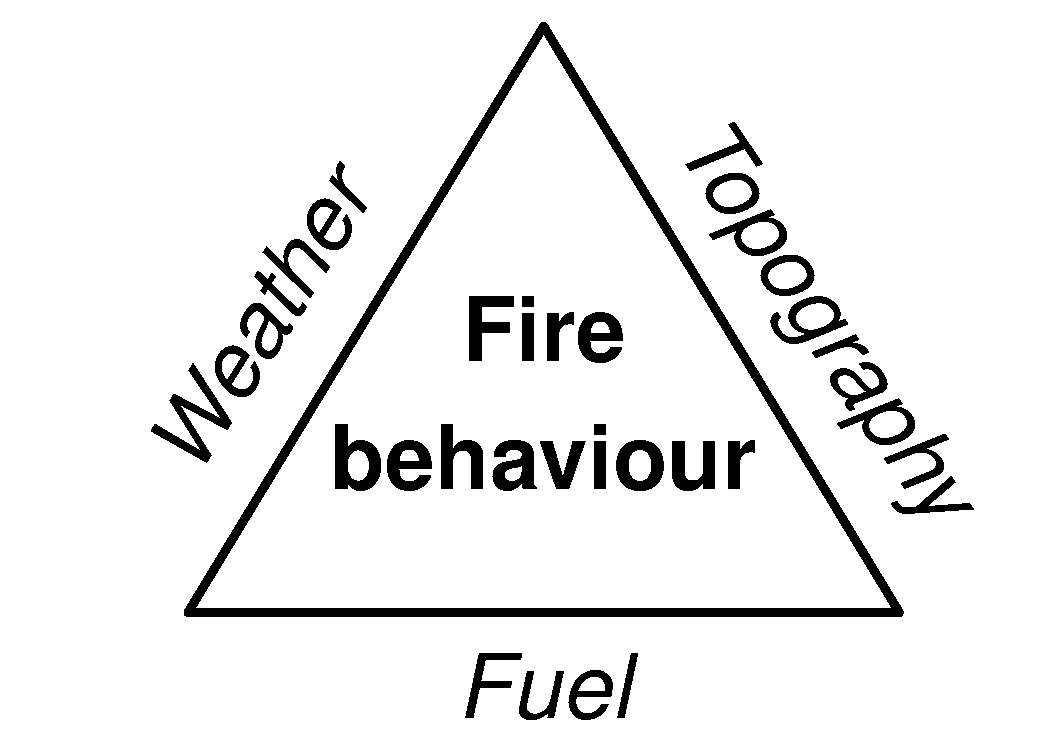
\includegraphics[width=2.2in, 
		trim={1.5cm 0cm 1cm 0.5cm}, clip=true]
		{science/behavior/FireBehaviourTriangle-1}
		\caption{Topography, weather, and the fuelbed are the three major drivers of wildland fire behaviour.
			\index{Fire triangles!Fire behaviour|textit} \label{fig:FireBehaviourTriangle} } 
		% (Fig.~\ref{fig:FireBehaviourTriangle})
	\end{center}
\end{marginfigure}

Weather, fuel, and topography all interact to determine the outcomes of fire spread \citep[][Fig.~\ref{fig:FireBehaviourTriangle}]{holsinger2016}.
Sampling fuels is discussed in Chapter~\ref{ch:fuels}, while weather measurement is discussed in Chapter~\ref{ch:weather}. 
Here we briefly review the role of topography. 

Fire moves more quickly upslope\textemdash and more slowly downslope\textemdash relative to flat ground, just as head fires move faster with the wind and backing fires more slowly against the wind. 
Because hot air rises, fuels on a slope above an actively-burning fire get a head start in pre-heating.\footnote{In fact, wind and slope are treated as \emph{additive factors} in many fire spread models, which means that their effects can generally be swapped for one another\textemdash what wind does to a fire on flat ground, slope will do about the same\textemdash or they can cancel each other out\textemdash a down-slope wind can move a fire downhill faster than it would move in the absence of wind.}

The implications for topography on prescribed fire management are perhaps more apparent than prescribed fire science. 
Managers must always take slope effects into account\textemdash especially when firing or staging equipment\textemdash and be able to foresee whether a strip laid at the bottom of a hill will rush upward faster than a torch operator might expect, or whether flames and smoke at the top of a hill will make control more difficult.

But all observers need to take note of the slope when making fire behavior observations. 
Consider how a steep slope might affect conclusions about a correlation made between fire behavior and fuel properties; flame length would be longer than those same fuel conditions on level ground. 
Thus, to the extent possible, slope effects should be controlled for by taking fire behavior observations on level ground.\footnote{ 
Although of course in some landscapes, level areas are the exception rather than the rule. In cases where it is inappropriate to \emph{control} for slope effects, they can be \emph{accounted} for by measuring the slope with an inclinometer or taking a precise GPS reading for the sample area and finding its slope later in a Digital Elevation Map in a GIS.}

\subsection{The role of temperature} 

First off, \textbf{does anything stand out as \emph{not} being discussed much in the list above?} 
Notice that no mention is made of temperature or heat, despite the obvious fact that fire is hot. 
It turns out that \emph{temperature}\textemdash defined as a measure of the average kinetic energy of the particles in a sample of matter\textemdash is actually a poor response variable to describe the behavior of fire in the wildland environment. 
Temperature has two major limitations: 
 
 \begin{itemize}[noitemsep]
 	\item \textbf{Temperature has no spatial or temporal component.} Consider an electric radiating space heater, plugged in and cranking out the same amount of heat energy each second it is turned on. 
 	How ``hot'' the heater feels depends on how close one is to it. 
 	Even if the heater were on wheels and moved across the room, ensuring every point in the room gets to be the same distance from the heating element at some point, the speed at which this process occurs is determined by an external force\textemdash maybe how hard someone is pushing the heater\textemdash that is not quantified by measuring the temperature. 
 	Similarly, the speed at which a flame front moves through a grassland depends on external factors\textemdash energy and moisture content of fuels, slope and wind\textemdash that are not reflected in the measurement of temperature at a given point at a given time. 
 	\item \textbf{Temperature is subject to the material measured.} How ``particles in a sample of matter'' move depends greatly on the properties of the material, irrespective of heat energy input. 
 	Even very close to the space heater, the kinetic energy of particles of asbestos insulation will respond much differently than a block of iron. 
 	In the wildland fire environment, the value of a temperature data point has almost as much to do with the properties of the device used to make the measurement as with the properties of the fire. 
\end{itemize}

Despite all of this, various measurements of temperature are probably the most frequently-reported data in the fire ecology literature. 
Temperature is intuitive and relatively easy to measure. 
Below, the discussion on measuring fire behavior focuses on using conventional methods to measure temperature in the wildland fire environment in new ways that increase the information value of the data they produce. 

\section{Measurement} 

Almost certainly, the most common device for measuring temperature in the wildland fire environment is the thermocouple.\footnote{
	Another common approach is the use of temperature-sensitive paints that discolor at various temperatures. 
	One can place heat-resistant tiles with a series of these paints before the fire, and by ascertaining which paints were distorted and which were not, one can narrow the range of temperature exposures down to the ranges tolerated by those paints.} 
The primary advantage of thermocouples over most other temperature sensors is that they can operate under exposure to extremely high temperatures, like wildland fire, and they aren't terribly expensive. 
But the thermocouple itself is a specific component; a thermocouple alone isn't enough to measure anything. 
In wildland fire science, the phrase ``we used thermocouples'' almost always refers to a system of thermocouples and the electronics necessary to process signals from the probes and record the data. 
Here we focus on each in turn. 

\subsection{Introducing the thermocouple}

\paragraph{The Seebeck effect}

The physics behind the thermocouple are pretty simple: When a wire is heated at one end, a temperature gradient forms along the wire and electrical signals are generated that can be detected at the other end. 
This is called the \emph{Seebeck effect}. 
The signals vary according to the material in the wire. 
Therefore, when two wires made of different metals are exposed to the same heat source, there is a detectable difference in their electrical responses. 
This difference scales predictably with the common temperature of the heated ends.
Thus, a thermocouple is simply two wires of different metals, joined at one end to detect temperature (the \emph{hot junction}), and ready to be connected to a device capable of detecting the signals at the other (the \emph{cold junction}). 
But as stated above, the detecting device is a separate part of the system. 
And even the wires are just conduits for the signal between the hot and cold junctions\textemdash apart from the heated tip, thermocouple wires are wrapped in thermal insulation to isolate all but the tip from heat exposure. 
Let's narrow our discussion down to the hot junction, the business end of the thermocouple. 

\subsubsection{Considerations at the hot junction} 

The hot junction can take various forms, with differences in their performance in the wildland fire environment (Fig.~\ref{fig:ProbeVsWire}). 
The differences arise from the varied applications of thermocouples\textemdash from residential thermostats to monitoring industrial furnaces and boilers.
In some cases, the hot junction consists of a \emph{probe}, a rigid sheath that encloses the wire connection. 
In other cases, the junction is simply a bare \emph{bead} in which a small weld, made to ensure the wires are connected, remains exposed just beyond the insulation.

\begin{figure} 
	\begin{center}
		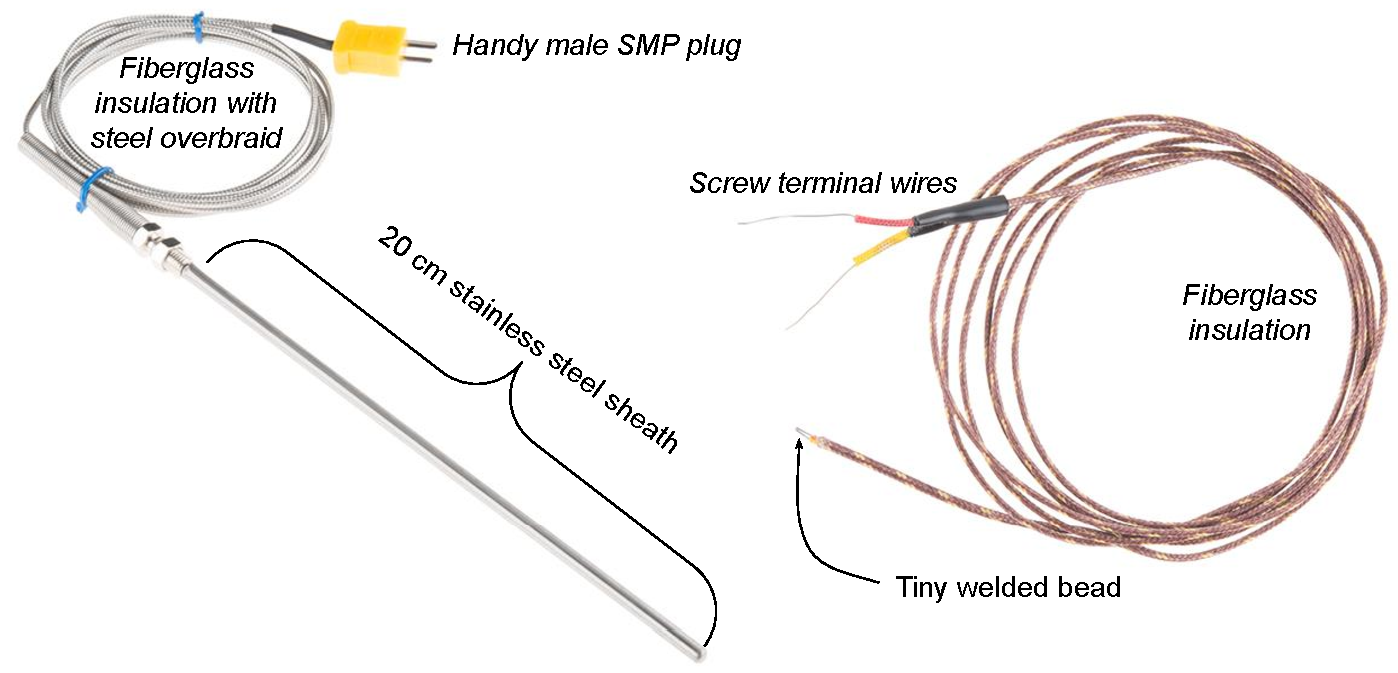
\includegraphics[width=1\textwidth]
		{science/behavior/TCcomparison}
	\ImageCredit{Modified from SparkFun.com, CC BY 2.0}
	\ImageIndex{CC BY 2.0}
	{fig:ProbeVsWire}
	{SparkFun.com}
	{https://www.sparkfun.com/categories/82}
	\end{center}
	\caption{Two types of hot junctions, with different thermocouple features identified. 
	On the left, the hot junction of a K type thermocouple is enclosed in a 20 cm $\times$ 5 mm stainless steel sheath. 
	On the right, the hot junction consists of a simple exposed welded bead.
	Note that all combinations of hot junctions, cold junctions, and everything in between are available. 
	} \label{fig:ProbeVsWire}
	%(Fig.~\ref{fig:ProbeVsWire})
\end{figure} 

Surprisingly, it does not appear that the relative merits of probes vs. beads for wildland fire science have been reported on, although the probe seems to introduce some confusion into what is actually being measured.\footnote{
	For example, \citet{coates2018} observed different temperatures from 28 cm probes laying horizontally along the soil surface to those standing vertically, which they attributed to the different ``orientation'' of the probes.
	But since the hot junction is at the end of probe, they've really just compared two points at different heights above the ground. 
	That temperature in the wildland fire environment changes with distance above the soil surface has been known for decades \citep[e.g.,][]{trollope1984}. }
The additional layer between the heat source and the hot junction introduced by the sheath might also complicate things. 
We suggest using exposed bead thermocouples. 

\paragraph{Realities of thermocouple measurements}
To place a thermocouple probe in the wildland fire environment is to subject it to all of the physical processes to which everything else in that environment is exposed. 
Thus, the same heat transfer dynamics apply to the thermocouple as to a fuel particle\textemdash simultaneous heating and cooling via convection, radiation, and conduction.\footnote{Let's assume the proper materials have been selected such that ignition and a phase change, i.e. melting, won't be issues for our sensor.}
This heat transfer is a combination of the properties of the media, the sensor, and the temperature gradient between them. 
A thermocouple placed 15 cm above the soil surface is responding to the kinetic energy of the air molecules around it. 
Likewise, a thermocouple placed in the soil is responding to the kinetic energy of the air, mineral, water, and organic matter molecules around it.
In each case, the sensor's response to changes in the media's kinetic energy has a lag time that reflects the mineral content and thickness of its materials, e.g., the wires themselves and welded bead or probe sheath. 

Thus, two realities that affect all thermocouple measurements include:\footnote{
	For a third reality, see Fig.~\ref{fig:FullHeatingCurves}.} 
 \begin{enumerate}[noitemsep]
	\item \textbf{Thermocouples always underestimate temperature.} 
	Like all particles in the wildland fire environment, the sensors are subject to cooling processes at the same time as they are subject to heating. 
	\item \textbf{Thermocouples are always at least a little bit behind in responding to changes.} 
	This lag time is often referred to as the thermocouple's \emph{response time}. 
\end{enumerate}

Wildland fire scientists have generally come to terms with each of these realities.
Regarding Reality 1, one assumes the recorded temperature is a relative value that scales consistently with the actual temperature; as such, for a researcher comparing measurements among different experimental groups, comparisons between observed temperatures are just as meaningful as if the actual temperatures are being compared.\footnote{
	When the true value is required, as can be the case in industry, two thermocouples of different diameters can be placed side-by-side and the actual temperature determined by extrapolating from the relative difference between the observed values \citep{walker1968}.} 
(Think of two parallel lines on a graph, with the same slope but different Y intercepts.)
Similarly, regarding Reality 2, fire scientists just try to use thin, responsive thermocouples and be consistent among observations so relative values can be used in place of actual heating rates and peak temperatures. 

While such work-arounds are often fine for comparisons within studies that use the same type of thermocouple, one encounters substantial barriers when trying to compare across studies that use different thermocouple set-ups (e.g., probe vs. bead, K-type vs. another type, different wire diameters, etc).
Imagine if other systems of measurement depended so much on the properties of the measurement device. 
Consider the frustration of using your ruler to determine you need a board 30 inches long and having the lumber yard cut one down for you using their ruler, only to find that it doesn't fit. 
It is already difficult enough to keep the units of length straight\textemdash inches vs. centimeters, yards vs. meters\textemdash it would be ridiculous if the same value resulted in different lengths because the measurements were made with two rulers of different thicknesses. 
But that is essentially the issue when comparing data collected with different thermocouple types.

\subsubsection{Signal processing and data logging}

Four basic but important steps occur on the other end of the thermocouple wires, at the cold junction: 
 \begin{itemize}[noitemsep]
	\item \textbf{Signal detection} Electrical signals in the wires are self-generated, so there is no power input required, but the voltage is low.
	\item \textbf{Reference temperature measurement} Converting the voltage differences in the wire to temperature requires the temperature of the cold junctions to be known. 
	\item \textbf{Temperature conversion} An equation is used to convert the voltage differences to temperature. 
	\item \textbf{Data storage} Most wildland fire science applications require thermocouple data\textemdash typically just a timestamp and temperature for each observation\textemdash to be stored for retrieval. 
\end{itemize}

Many instruments are designed to operate thermocouples and most take care of all of the above steps internally. 
But there are several discrete functions being performed, and variability in each dictate the nature of the systems available to the user:\footnote{Understanding this variability allows the user to select or even assemble systems that focus on getting the right type of performance for a given budget.}
 \begin{itemize}[noitemsep]
	\item Voltages are very low and quality electronics often amplify incoming signals.
	\item Devices typically include a basic semiconductor thermometer to ascertain reference temperatures.
	\item Conversion equations are specific to the metal in the wires, so devices are either limited to the type of thermocouple they are compatible with or require the user to identify the thermocouple via software interface.
	\item Data storage requires either a removable card slot or onboard media and some means to interface with it. 
	\item Integrated systems require a computer or microprocessor to coordinate all of these tasks, which in turn requires a power source (even though the signals from the Seebeck effect are self-generated!). 
\end{itemize}

Here we review three broad categories of electronics available to the wildland fire scientist:\footnote{
	Note that reference to trade names or specific commercial products are not product endorsements, but are used only as examples.}

\paragraph{Basic thermocouple dataloggers} 

Among the lowest-cost options for thermocouple electronics are self-contained devices into which one plugs a thermocouple and downloads the data to a computer afterwards. 
Popular commercial solutions include HOBO\textregistered{} products from the Onset Computer Corporation (\href{www.onsetcomp.com}{onsetcomp.com}; Bourne, MA), which include single-channel (one thermocouple per datalogger) and four-channel (four thermocouples per datalogger) options that have been updated to include real-time visual displays of temperature and memory and battery capacity (earlier versions where just little white buttons with an on switch and a blinking light). 
These devices are programmed, and their data accessed, via proprietary but zero-cost software. 

\begin{itemize}[noitemsep]
	\item \textit{Advantages:} Relatively low-cost and easy to operate; small and easy to protect from heat exposure; most compatible with a wide range of thermocouple types.  
	\item \textit{Disadvantages:} Still not cheap (US\$150 or 305, 1 or 4 channels; logger only); use limited to logging temperature from thermocouples; restricted proprietary software for both operation and interface.
\end{itemize}

\paragraph{Multi-purpose dataloggers with thermocouple capacity}
Of course, the scientific and industrial worlds\textemdash and thus many lab cabinets\textemdash are full of datalogger options for applications that go way beyond wildland fire. 
Most users might not appreciate how many functions are included in the catch-all term ``datalogger,'' which includes an onboard processor and several input/output options. 
Almost any microprocessor-driven datalogger system can be made compatible with thermocouples\textemdash thermocouple-unique tasks are the signal amplification and a program with the voltage-temperature conversion equation. 
Many such systems are commercially available and ready for thermocouples out of the box. 
For example, almost every CR model from Campbell Scientific (\href{https://www.campbellsci.com/data-loggers}{campbellsci.com}; Logan, UT) will handle many types of thermocouples (Fig.~\ref{fig:cr1000}). 

\begin{marginfigure}
	\begin{center}
		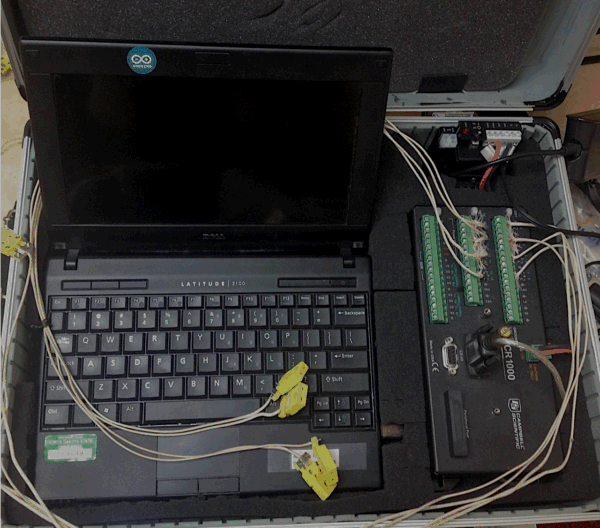
\includegraphics[width=2.2in]
		{science/behavior/CR1000}
		\caption{A Campbell Scientific CR1000 datalogger set up to read 8 thermocouple leads. 
		While onboard data storage is available for CR dataloggers, this system is set up to display realtime data and write to the laptop via proprietary CS software.  
			\label{fig:cr1000} } 
		% (Fig.~\ref{fig:cr1000})
	\end{center}
\end{marginfigure}

\begin{itemize}[noitemsep]
	\item \textit{Advantages:} Versatile systems for applications beyond fire science that include options for remote connectivity; often capable of handling many channels efficiently; usually many options for interface and data storage; often have more flexible programming options.   
	\item \textit{Disadvantages:} More\textemdash sometimes much more\textemdash expensive; often larger and more difficult to protect from heat exposure; often limited to proprietary programming languages.
\end{itemize}

\paragraph{Open-source DIY electronics systems}
Just as corporations like Onset and Campbell Scientific started with someone tinkering with electronics to accomplish a task, individual users can assemble their own custom systems based on low-cost parts running open-source code. 
The rise of the Maker's Movement and global connectivity via the Internet has produced many products and a community of developers relevant to wildland fire science. 
In particular, the low-cost, open-source Arduino platform (\href{http://www.arduino.cc}{arduino.cc}) is very user-friendly and accessible even to n00bs. 
In its most basic form, the Arduino system offers cheap microprocessors programmable via a free variant of the classic \texttt{C++} language (Fig.~\ref{fig:DIYboards}, \emph{top}). 
As long as one isn't afraid to solder and code, there is hardly a limit on what the wildland fire scientist can build to custom specifications for a fraction of the cost of commercial systems. 

\begin{marginfigure}
	\begin{center}
		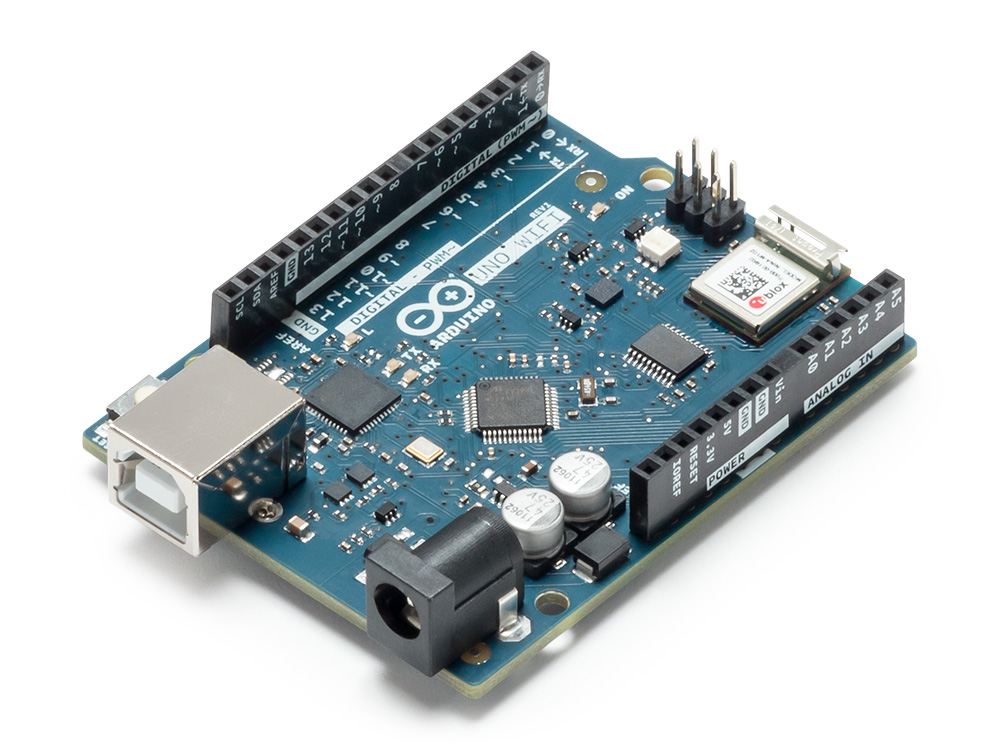
\includegraphics[width=2.2in]
		{science/behavior/ArduinoUno}
		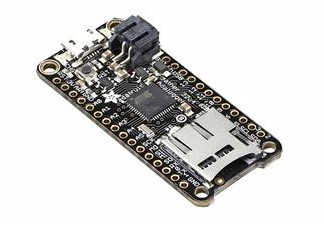
\includegraphics[width=2.2in]
		{science/behavior/AdaLogger}
		\caption{Two examples of open-source, DIY microprocessor systems. 
			Top: A basic Arduino Uno. 
			Bottom: A Feather M0 Adalogger from Adafruit Industries, with USB connections, JST battery terminal, and onboard $\mu$SD card slot. 
			Both systems are programmed with a variant of \texttt{C++}; light versions of Python are available as well.
			\label{fig:DIYboards} } 
		% (Fig.~\ref{fig:DIYboards})
	\end{center}
\end{marginfigure}

The Arduino-adjacent Feather family of microcontroller products and peripherals from Adafruit Industries (\href{http://www.adafruit.com}{adafruit.com}; Brooklyn, NY) is particularly well-suited for wildland fire science because it is designed for mobility\textemdash small components that run on relatively small batteries (Fig.~\ref{fig:DIYboards}, \emph{bottom}). 
The FeatherFlame system \citep[][\href{https://www.diyfirescience.info}{diyfirescience.info}]{mcgranahan2021b} combines Adafruit products to amplify and process signals from up to 6 K-type thermocouples and store the data on a removable microSD card. 

\begin{itemize}[noitemsep]
	\item \textit{Advantages:} Maximum versatility in both hardware and software; often cheapest options available; small and easy to protect from heat exposure (and cheaper to replace).   
	\item \textit{Disadvantages:} Assembly required, and no customer support\textemdash following published projects requires basic soldering and coding skills, while substantial project customization and design require moderate skills in circuitry and coding; materials are developed for hobbyists and STEM classrooms and might not have the longest life in rugged conditions.
\end{itemize}

\section{Thermocouple deployment} 

Where does one put thermocouples out in the landscape? 
The answer starts with the purposes of the data collection in the first place\textemdash who wants to know what about fire behavior? 
If some specific fire effects are going to be measured, it makes sense to place sensors near where those measurements will be taken, or where the heat input will occur: If one is studying grass bud mortality, one might put a thermocouple in the crown of the grass plant; if one is concerned about soil microbe mortality, thermocouples can be placed at or even below the soil surface. 
If general fire behavior measurements are desired, it is easy to use thermocouples to measure rate of spread by placing clusters in representative areas of the fuelbed. 
 
 \begin{marginfigure}
	\begin{center}
		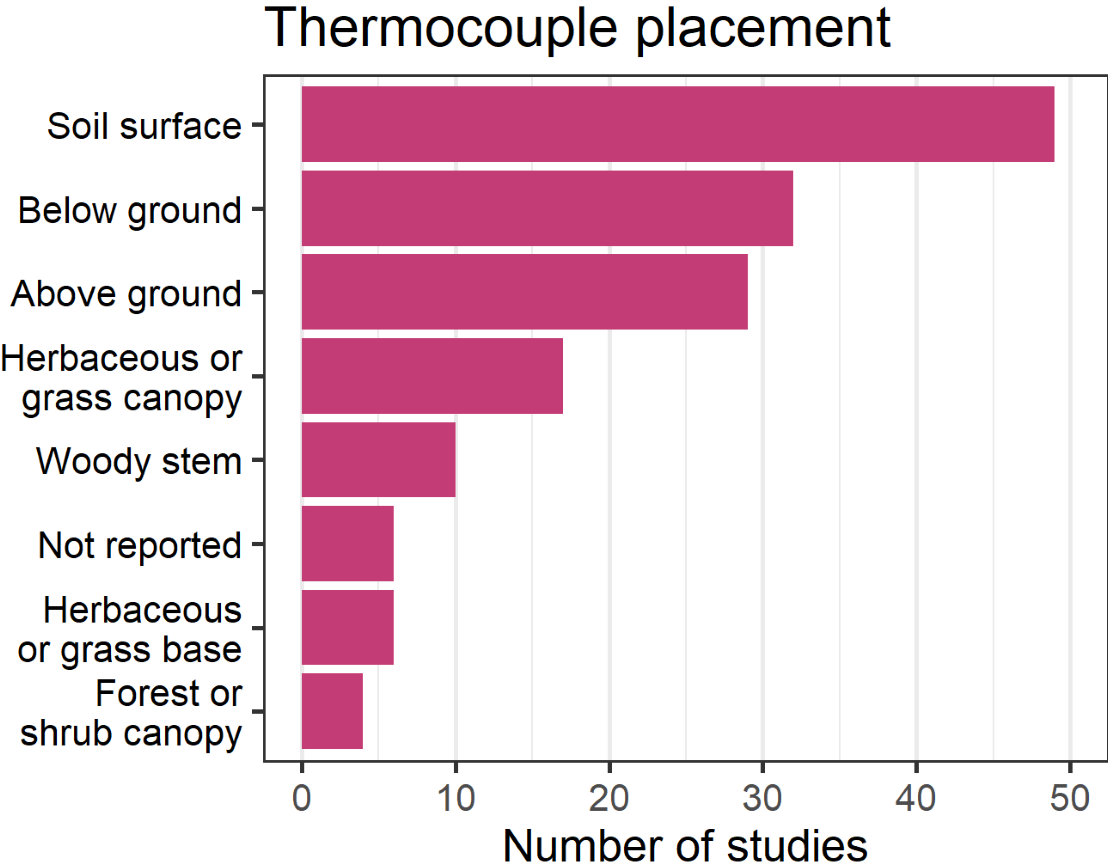
\includegraphics[width=2.2in]
			{science/behavior/placement}
		\ImageCredit{\citet{mcgranahan2020}}
		\caption{Frequencies of various locations thermocouples were deployed in the wildland fire environment, based on a review of 105 studies. 
		\label{fig:placement} } 
		% (Fig.~\ref{fig:placement})
	\end{center}
\end{marginfigure}

The primary considerations are vertical and horizontal: At what height to put thermocouples, and how far apart? 
Unfortunately there are no standard protocols to guide either. 
Among published studies, the most common placement is right on the soil surface, followed by placements above the ground and somewhere above the ground (Fig.~\ref{fig:placement}). 
There is no standard for the height of aboveground placement, even though studies that report values for multiple intervals above the ground show wide variability. 
In terms of best capturing the ``hottest'' part of the vertical flame profile, something like 50\% of the overall height of herbaceous fuelbeds is probably most appropriate. 
Heights like 15 or 20 cm are common in grassland fuels. 
 
In terms of horizontal arrangement, many thermocouple sampling designs are limited by the number of thermocouples available, and just a handful are deployed per burn with little attention to their spacing. 
But if thermocouples are thoughtfully arranged, it is possible to analyze data in a manner that provides much more information on fire behavior than temperatures alone. 
Specifically, when thermocouples are spaced at known distances, the timestamps can be determine when flame fronts arrived at each sensor, and thus how quickly the flame front moved between sensors\textemdash \emph{rate of spread}.   

There are two options for measuring rate of spread with time-temperature data from thermocouples \citep{finney2021}:

\emph{One-dimensional spread} measures the linear rate of spread along a transect and is best measured under direct visual observation \citep{cruz2020}.
This is a common technique applied to specific parts of the fire, such as comparing head fire and back fire spread.\footnote{
	Fire behavior analysts often focus on head fires, specifically, because the \emph{forward rate of spread} is a common output for fire behavior models and is most pertinent to tactical decisionmaking.}
The technique requires knowing wind direction and the type of fire moving along the transect, and is most accurate when the angle of spread aligns with the angle of the transect. 

\emph{Two-dimensional spread} requires neither knowing the wind direction nor alignment between sensor points and flame front.\footnote{
	While this technique does not require direct observation, determining what type of fire spreads through the array is best determined visually.} 
Instead, trigonometry is used to determine spread through a non-linear array of sensors.
When thermocouples are arranged in equilateral triangles such that individual sensors share common timestamps\textemdash as when connected to a multi-channel datalogger\textemdash one can calculate rate of spread through the array \citep{simard1984, kidnie2015a}.
One can also nest several smaller equilateral triangles, or \emph{microplots}, in a spatially-hierarchical design that facilitates geospatial analysis of fuel and fire behavior patterns (Fig.~\ref{fig:SierpinksiTriangle}). 

\begin{figure} 
	\begin{center}
		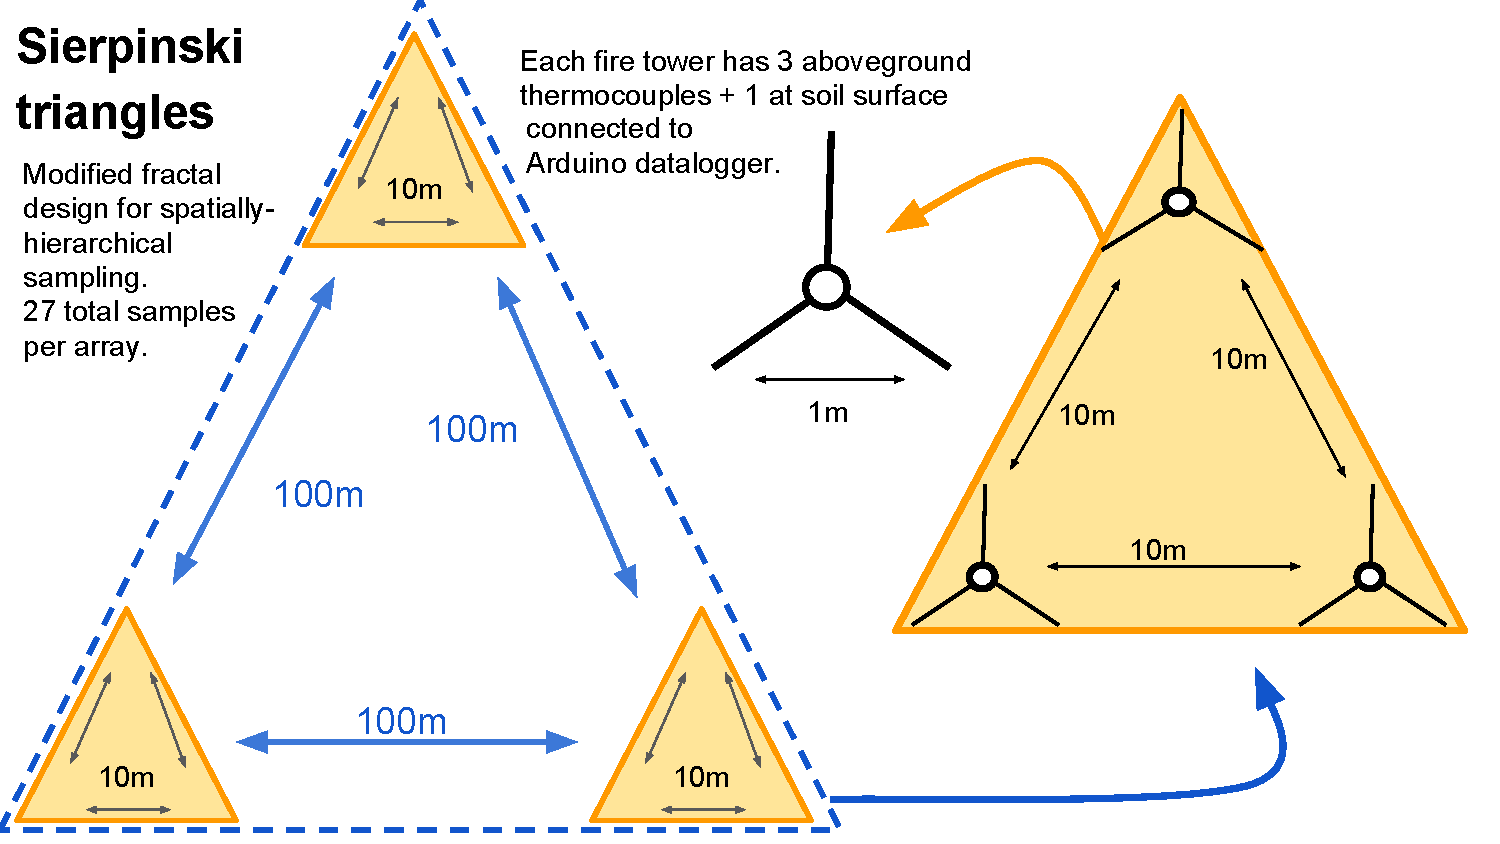
\includegraphics[width=1\textwidth]
			{science/behavior/SierpinskiTriangle}
	\end{center}
	\caption{An example of an spatially-hierarchical arrangement of thermocouple sensors \citep{mcgranahan2021b}.
		Each  1m equilateral triangle represents a \emph{microplot} for which rate of spread can be determined; the fractal design of the Sierpinksi Triangle is intended to facilitate spatial analysis of patterns in fuel and fire behavior across multiple scales. 
	} \label{fig:SierpinksiTriangle}
	%(Fig.~\ref{fig:SierpinksiTriangle})
\end{figure}

In plot-based studies ignited by a rapid ring ignition pattern, it is possible to calculate rate of spread based on the time taken for fire to spread through the entire plot \citep[e.g.,][]{trollope1985}.
Such a method does not require any equipment more fancy than a stopwatch.   

\section{Processing thermocouple data} 

\subsection{From logger to workspace} 

Raw thermocouple data are often a mess\textemdash mere seconds of meaningful data as the flame front passes buried in hours of ambient temperature records. 
But it is difficult to automate the extraction process because noise is often introduced into the data file (Fig.~\ref{fig:RoughWindows}, \emph{top}). 
\href{https://diyfirescience.info/portfolio/heatingcurvescript/}{This blog post} describes how to use the \href{https://www.r-project.org/}{\textbf{R}} statistical environment to identify ``rough windows'' within the time-temperature curves for extraction (Fig.~\ref{fig:RoughWindows}, \emph{bottom}). 
Within these windows, minimum values, maximum values, and the data in between can be more reliably attributed to heating processes at the hot junction than noise at the cold junction. 

\begin{figure} 
	\begin{center}
		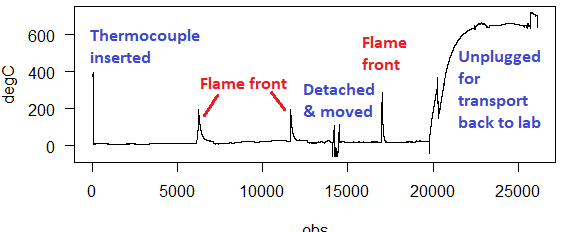
\includegraphics[width=1\textwidth]
			{science/behavior/HoboExample} \\
		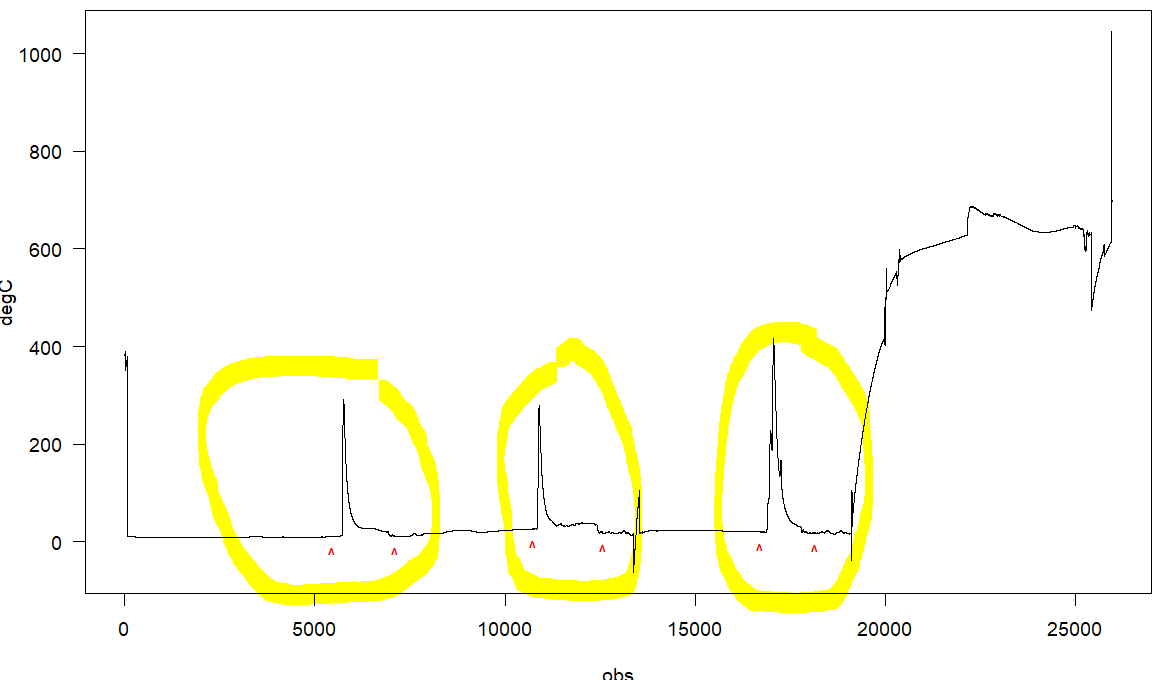
\includegraphics[width=1\textwidth]
			{science/behavior/ClickCapture}
	\end{center}
	\caption{Top: An example of three meaningful heating events buried in hours of noisy data from a HOBO datalogger. 
		Note that data associated with the heating events are never the highest or lowest values in the series. 
		Bottom: Rough windows around heating events identified with \href{https://diyfirescience.info/portfolio/heatingcurvescript/}{an R script.} 
	} \label{fig:RoughWindows}
	%(Fig.~\ref{fig:RoughWindows})
\end{figure}

\subsection{Analysis}

\begin{marginfigure}
	\begin{center}
		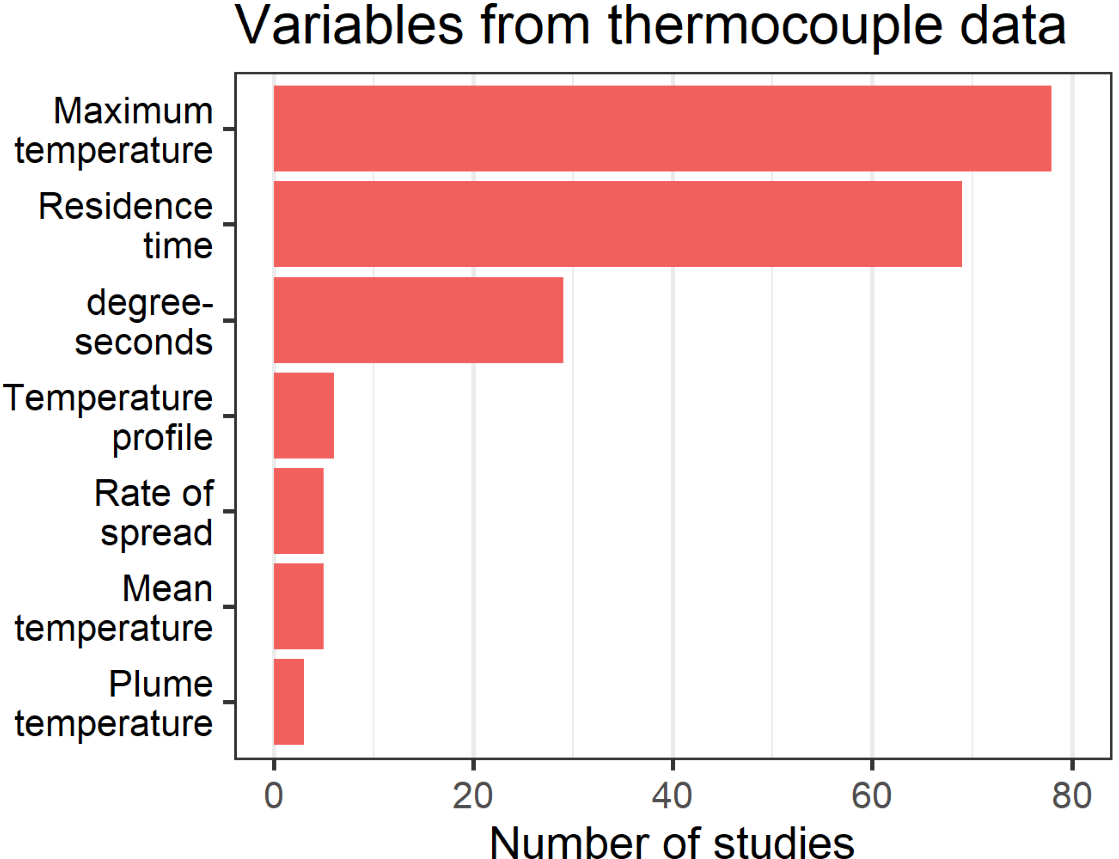
\includegraphics[width=2.2in]
			{science/behavior/TCresponses}
		\caption{Frequencies of various response variables derived from thermocouple data, based on a review of 105 studies \citep{mcgranahan2020}. 
			\label{fig:responses} } 
		% (Fig.~\ref{fig:responses})
	\end{center}
\end{marginfigure}

Because thermocouples measure temperature and fire is hot, it is not surprising that the most commonly-reported response variable from thermocouple data is maximum temperature (Fig.~\ref{fig:responses}). 
But leveraging the \emph{time} component of thermocouple data, rather than \emph{temperature}, allows one to calculate less subjective measures of fire behavior. 
For example, rate of spread data can be combined with the other parameters in Eq.~\ref{eq:byram} to estimate intensity, and sidestep all of the issues around trying to use temperature as a fire response variable.   

\subsubsection{2-D rate of spread} 

With foresight in thermocouple deployment, it is possible to calculate rate of spread without knowing its direction. 
To facilitate measuring two-dimensional rate of spread, \citet{simard1984} provided a series of equations that use trigonometry to calculate how fast a flame front moved through an array laid out as an equilateral triangle with sides $D$:

Let $t_1$, $t_2$, and $t_3$ represent arrival times\footnote{
	There are a couple of approaches to determining arrival times, e.g., the timestamp for the first record of some level of heating (\citet{kidnie2015a} used 300\degC), or peak temperature \citep{mcgranahan2021b}.} of flame fronts at vertices of equilateral triangle.
If $t_1 \neq t_2$,

\begin{equation} \label{eq:simard1}
	\theta = tan\textsuperscript{-1} \left( \dfrac{2t_3 - t_2 - t_1}{\sqrt{3}\cdot (t_2 - t_1)}\right) 
\end{equation}

and rate of spread $r$ is 

\begin{equation} \label{eq:simard2}
	r = \dfrac{D\cdot cos\theta}{t_2 - t_1}
\end{equation}

otherwise, if $t_1 = t_2$, $\theta = 90$ and rate of spread $r$ is 

\begin{equation}\label{eq:simard3}
	r = D (\sqrt{3}/2)/({t_3 - t_1})
\end{equation}

\subsubsection{Heating curves}

\begin{marginfigure}
	\begin{center}
		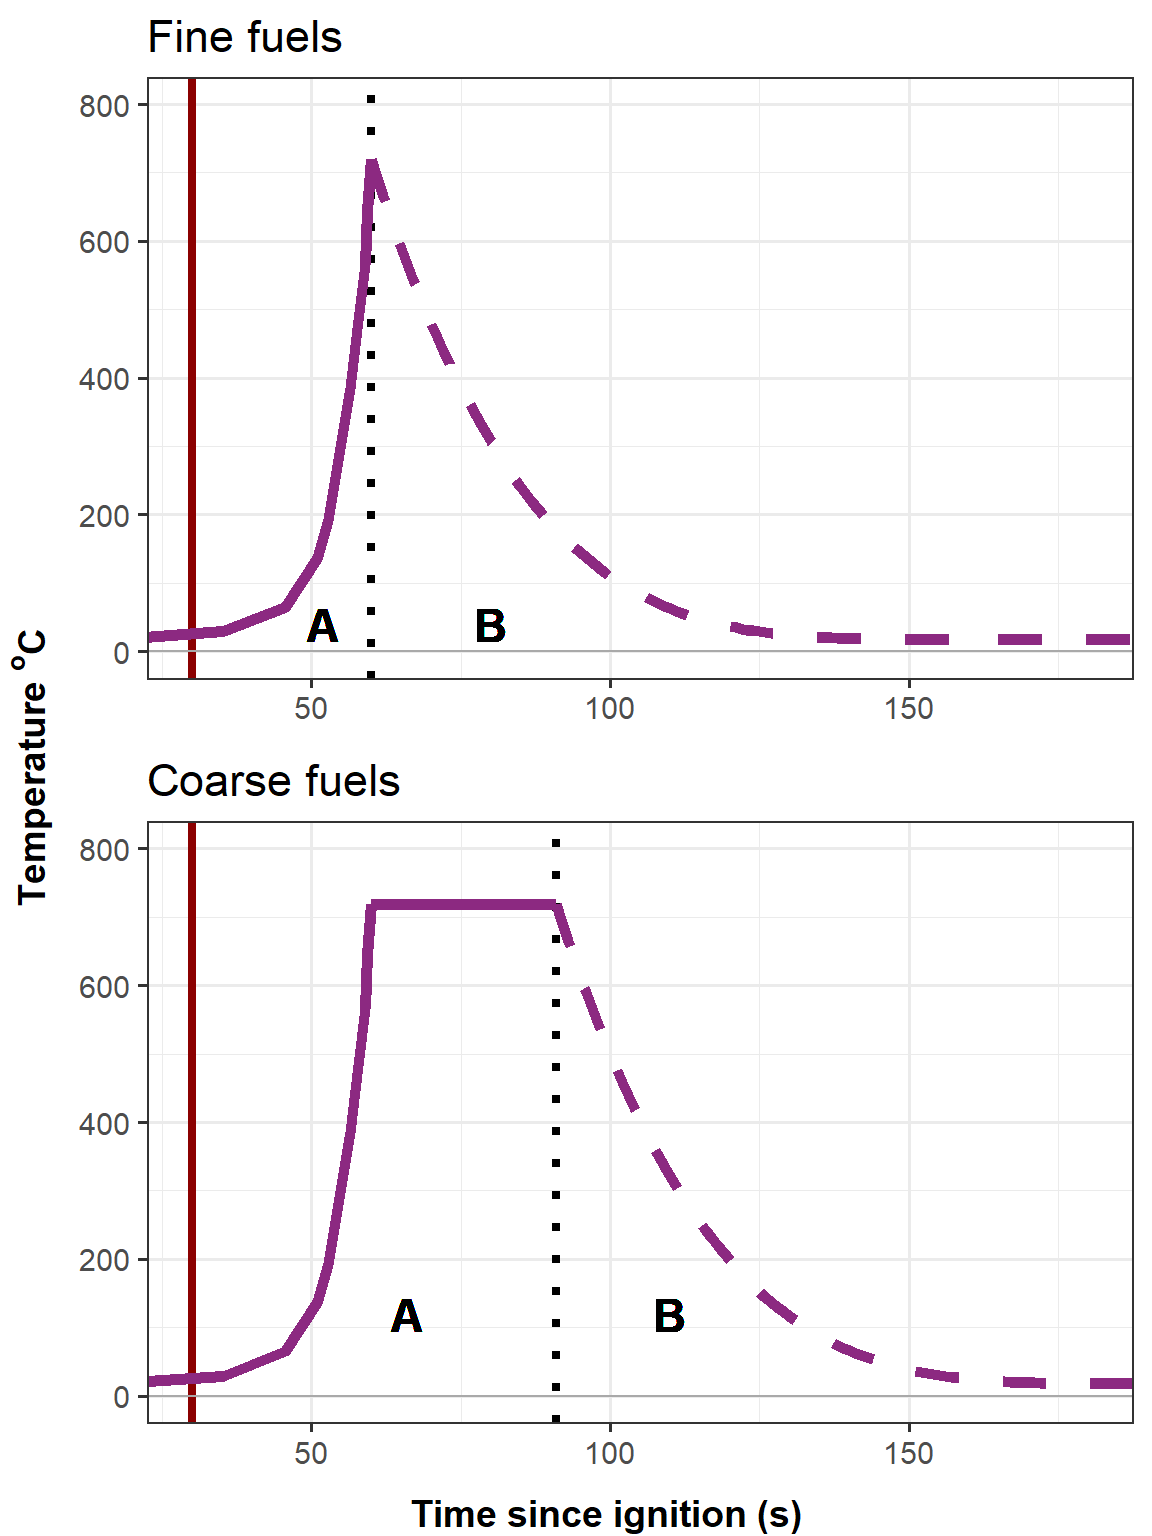
\includegraphics[width=2.2in]
		{science/behavior/FullHeatingCurves}
		\caption{Examples of heating curves described by time-temperature data from fine and coarse fuels. 
			While many ecologists use the entire curve to calculate heat dose, \citet{mcgranahan2020} describe how including the cooling portion of the curve (dashed segments) is a mistake because that reflects the cooling of the hot junction, not the physical presence of heat energy in the fire environment. 
			Proper calculations of heat dose really ought to focus on the heating portion by truncating the time-temp data at the point it begins to reflect cooling (broken vertical black line). 
			\label{fig:FullHeatingCurves} } 
		% (Fig.~\ref{fig:FullHeatingCurves})
	\end{center}
\end{marginfigure}

Fire ecologists often calculate a \emph{heat dose} from thermocouple data that is intended to represent the amount of heat an organ, organism, or soil stratum is exposed to (Fig.~\ref{fig:responses}). 
Time-temperature curves are ideal data for doing so, although unfortunately the data are often misapplied in calculations of heat dose (we aren't going to get into here, but see fig.~\ref{fig:FullHeatingCurves} for a summary of the issue).

Once the beginning and end points of the heating curve are determined from the ``rough windows'' described above, one can extract several parameters useful for further analyses (Fig.~\ref{fig:HeatingCurve}). 
The heat dose is obtained by integrating the area under the heating curve \citep[e.g.,][]{engle1989}. 
Beginning temperatures and rate of heating are useful parameters in soil heating models. 

\begin{figure} 
	\begin{center}
		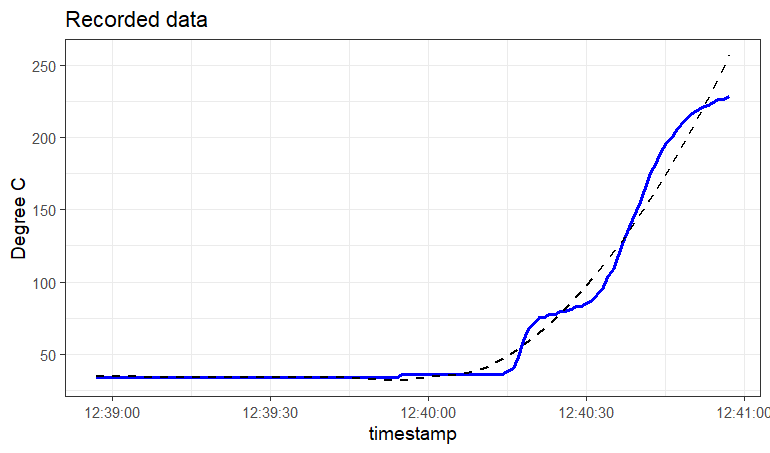
\includegraphics[width=1\textwidth]
		{science/behavior/RecordedData} \\
		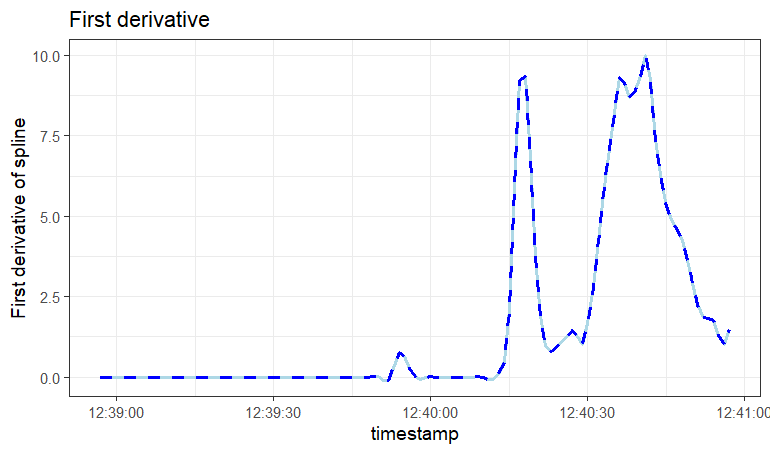
\includegraphics[width=1\textwidth]
		{science/behavior/FirstDerivative} \\
		\includegraphics[width=1\textwidth]
		{science/behavior/heatingCurve} \\
		\begin{tabular}{ccccc}
			\hline
			Start $^\circ C$ & Max $^\circ C$ & s to Max $^\circ C$ & Rate ($^\circ C~s^{\text{-}1}$) & Heat dose \\ 
			\hline
			34.4 & 228.4 & 1.1 & 181.9 & 6410.6 \\ 
			\hline
		\end{tabular}
	\end{center}
	\caption{An example of steps to calculate parameters from heating curves. 		Top: A smoothed spline fit to the raw data from the rough window. Center: The first derivative of the smoothed spline identifies the point at which heating begins. Bottom: The curve is trimmed to begin at the first non-zero positive first derivative and a logistic curve fit to the raw data, under which the area is integrated between the endpoints of the heating curve. Table: Examples of heating parameters extracted from the final curve.  }
	\label{fig:HeatingCurve} 
	%(Fig.~\ref{fig:HeatingCurve})
\end{figure}
